\documentclass[11pt]{book}

\usepackage{html}
\usepackage{hypre}
\usepackage{makeidx}
\usepackage{graphicx}

%=============================================================================
% Preamble:
%=============================================================================

% set margins
\setlength{\oddsidemargin}{0in}
\setlength{\evensidemargin}{0in}
\setlength{\textwidth}{6.5in}
\setlength{\topmargin}{0in}
\setlength{\textheight}{8.0in}

% define various commands and macros

% define the version number
% NOTE: this is automatically generated from another file in hypre
\def\HYPREVersion{2.4.0b}
\def\HYPREVersionDate{2008/08/08}


% write out the index entries in the `.idx' file
\makeindex

%=============================================================================
% Body:
%=============================================================================

\begin{document}

%=============== Title Page

\begin{TitlePage}

\Title{Developer's Manual}
\SubTitle{Software Revision: \HYPREVersion}
\SubTitle{Date: \HYPREVersionDate}
\vfill
\begin{center}
\InsertGraphics{hypre_wiw}{width=.7\textwidth}
\end{center}
\vfill
\Author{%
Center for Applied Scientific Computing\\
Lawrence Livermore National Laboratory
}

\end{TitlePage}

%=============== Copyright Page

\begin{CopyrightPage}
\noindent
Copyright (c) 2006   The Regents of the University of California.
Produced at the Lawrence Livermore National Laboratory.
Written by the HYPRE team, (hypre-users@llnl.gov), UCRL-CODE-222953.
All rights reserved.

\vspace{1em}\noindent
This notice is required to be provided under our contract with the U.S. 
Department of Energy (DOE). This work was produced at the University of 
California, Lawrence Livermore National Laboratory under Contract No. W7405-ENG-48 with the DOE.
 
\vspace{1em}\noindent
Neither the United States Government nor the University of California nor any 
of their employees, makes any warranty, express or implied, or assumes any 
liability or responsibility for the accuracy, completeness, or usefulness of any 
information, apparatus, product, or process disclosed, or represents that its use 
would not infringe privately-owned rights. 

\vspace{1em}\noindent
Also, reference herein to any specific commercial products, process, or 
services by trade name, trademark, manufacturer or otherwise does not 
necessarily constitute or imply its endorsement, recommendation, or favoring by 
the United States Government or the University of California. The views and 
opinions of authors expressed herein do not necessarily state or reflect those of 
the United States Government or the University of California, and shall not be 
used for advertising or product endorsement purposes. 

\vspace{1em}\noindent
This file is part of HYPRE (see http://www.llnl.gov/CASC/hypre/).
Please see the COPYRIGHT\_and\_LICENSE file for the copyright notice, 
disclaimer and the GNU Lesser General Public License.

\vspace{1em}\noindent
This program is free software; you can redistribute it and/or modify it
under the terms of the GNU General Public License (as published by the Free
Software Foundation) version 2.1 dated February 1999.
  
\vspace{1em}\noindent
This program is distributed in the hope that it will be useful, but WITHOUT
ANY WARRANTY; without even the IMPLIED WARRANTY OF MERCHANTABILITY or
FITNESS FOR A PARTICULAR PURPOSE.  See the terms and conditions of the
GNU General Public License for more details.

\vspace{1em}\noindent
You should have received a copy of the GNU Lesser General Public License
along with this program; if not, write to the Free Software Foundation,
Inc., 59 Temple Place, Suite 330, Boston, MA 02111-1307 USA

\end{CopyrightPage}

%=============== Table of Contents

\pagenumbering{roman}
\tableofcontents
\cleardoublepage
\pagenumbering{arabic}

%=============== Include Chapters

%==========================================================================
\chapter{\hypre{} Requirements}
\label{hypre Requirements}

%==========================================================================
\section{Functional Requirements}
\label{Functional Requirements}

\begin{description}

\item[R1] \hypre{} will consist of a set of linear solvers,
preconditioners, libraries of linear solvers, and an interface that
allows various applications to use these libraries and linear solvers
in various ways.
\begin{description}

\item[R1.1] Current linear solver include ILUT, AMG, EBE, PILUT, SMG,
and

\item[R1.2] Current libraries of linear solvers include PetsC, ISIS, and

\end{description}

\item[R2] \hypre{} must allow access to other libraries of linear
solvers directly through the \hypre{} interface and allow \hypre{}'s other
linear solvers and preconditioners to be accesses via the standard
interface for the other libraries of linear solvers.


\item[R3] New linear solvers, preconditioners, and libraries of
linear solvers should be able to be added to \hypre{} and accessed
through the \hypre{} interface any time without much modification.
\begin{description}

\item[R3.1] A degree of modularity and loose coupling should exist to
ensure modification and enhancements are simple.

\item[R3.2] (related to R2 also): every linear solver and
preconditioner should exist independently of the \hypre{} interface.

\end{description}

\item[R4] The applications that will use \hypre{} may provide data in a
variety of forms.  \hypre{} should allow new forms of data to be input
without much modification.
\begin{description}

\item[R4.1] Currently application data may consist of linear algebra,
finite elements, stencils, and

\item[R4.2] The \hypre{} interface should be modular to the extent that
adding new valid application data forms will be simple.

\end{description}

\item[R5] \hypre{} should provide mechanisms to maximize the number of
linear solvers and preconditioners avialable to an application
regardless of the format of that data provided by those applications.
\begin{description}

\item[R5.1] The user will choose which linear solver or preconditioner
to apply to the data. (A set of valid choices will be provided).

\item[R5.1] This should be accomplished primarily by "translating"
the application data into the storage schema required by the solver or
preconditioner or by applting the coefficient access method required
by the solver or preconditioner.

\end{description}

\end{description}

%==========================================================================
\section{Non-Functional Requirements}
\label{Non-Functional Requirements}

\begin{description}

\item[R6] \hypre{} should be portable across these platforms: Sun, DEC,
BLue, and
	
\item[R7] \hypre{} should work with applications written in C, C++,
FORTRAN77, and
	
\item[R8] \hypre{} should should be easy to compile, configure, and
install.

\item[R9] \hypre{} should be scalable.

\item[R10] \hypre{} should work with applications that utilize the MPI
standard as well as those incorporating both MPI and OpenMP or MPI and
Pthreads.

\end{description}


%==========================================================================
\chapter{Design}
\label{Design}

%==========================================================================
\section{Software Architecture}
\label{Software Architecture}

\subsection{More detail on the programming model}


\hypre{} is more than just a
library of solver routines: it 
is actually a collection of pieces that can be "programmed" in different ways.
Technically speaking, 
\hypre{} is a "component model." It is not necessary to have any formal training
in "components" to be able 
to use \hypre{}, however. In our experience, looking at some examples and
programming a simple example 
or two quickly gives users an intuitive feel for how this model works. In
brief, the major "mental shift" 
necessary is to accept that \hypre{} represents all of the parts of a linear
solver library as "encapsulated 
objects", called "components". This includes the obvious candidates such as
matrices, but also the less 
obvious things such as the algorithms used to implement preconditioning. Each
object is opaque and can be 
used only through the advertised "services" that it supports. All function
calls within \hypre{} are 
considered to be a function "of some object/component", and the functions that
work on a particular 
component are exactly the set of "services" that that component provides. In C
language, that component is 
always the first parameter in the function call, for example. Other parameters
in a function call are normal 
parameters, but the first one is always the component that the function call is
"acting on". The list of 
services provided by each component are easily discovered by looking at the
header files for each 
component, as well as other centralized documentation. 

In many ways, the ``component design'' of HYPRE is simpler than object-oriented
design, and it can be explained in an analogy to traditional subroutine
libraries.
As mentioned above, there are two entities in HYPRE: lists of services, and
pieces of software that implement some subset of those services.
This is a direct analog of old-fashioned procedural libraries, for example,
the Basic Linear Algebra Subroutine (BLAS): the ``lists of
services'' are the functions that a library might implement, and the pieces
of software that implement the services are the specific library implementations.
The BLAS are not an exact fit to this analogy, because typically a library
that implements part of the BLAS implements it all.
Imagine, though, that different BLAS libraries implemented only the portion
of the BLAS that the developers chose to implement, either due to manpower,
area of expertise, interest, need, etc.
As a user, the way you would use such a system would be to figure out which
functions you want to call (i.e. which services you would like to use), make
a call to that routine in your program, and then look at all of the available
BLAS implementations to find the ones that have implemented the call that you
made and choose one.
One way to think about HYPRE is exactly analagous: the BLAS functions are 
the analog of the abstract interfaces within HYPRE, and the analog of a BLAS
library is a particular HYPRE component.

Besides for the services that a component provides, there is only one other use
of a given component within 
\hypre{}, and that is as an input to other components. For example, \hypre{} provides
several components 
that implement preconditioning algorithms. A user may very well set up a
preconditioner but never call any 
services from the preconditioner directly. Instead, the preconditioner is
handed to a solver within \hypre{} 
and the solver uses that preconditioner. Thus, the way to decide if you want to
use a particular component 
is to ask "do I want to use any of its services" and "do I need it as input to
another component that I want to 
use?" If the answer to either question is "yes", then you need that component.

The components are then put together as inputs to each other to collaborate on
performing the desired 
action. The "desired action" is typically the solution of a single linear
system of equations and \hypre{} is 
specialized to make that extremely easy, but one of the benefits of \hypre{}'s
programming model is that 
the parts can be combined together in different ways to perform different
actions. Examples might be: 
reusing preconditioners over several timesteps of a time-dependent calculation,
using a solver as a 
preconditioner, or providing user-defined matrices or preconditioners for use
within \hypre{}. Generally, 
these more complex usages are performed by more expert users, including
developers of other solver 
components.


%==========================================================================
\section{Object Model}
\label{Object Model}


{\bf Abstract versus concrete types:} 

In the current version of HYPRE, we use a capitalization scheme
to differentiate types in 
\hypre{}: capital \code{HYPRE} refers to abstract classes, that is, services,
while lower \code{hypre} refers to concrete classes. 
If you
declare something to be of 
type \code{HYPRE_Solver}, for instance (see declaration of components below), it is
equivalent to stating that you 
will be using a component that supports the services listed in the 
\code{HYPRE_Solver}
class. On the other hand, 
lowercase \code{hypre} indicates a specific component, that is, a "concrete class".
The \code{hypre_StructSMGSolve}r, 
for instance, is a particular component. Just as in object-oriented libraries,
"upcasting" is always allowed. 
This means that in the bulk of your program code, you can refer to components
as if they were the abstract 
types. Only in the declaration of the component is the concrete class
mentioned. This technique is 
invaluable for promoting plug and play. In this example, then, you could
declare 

\begin{display}
\begin{verbatim}

HYPRE_Solver A; 
hypre_StructSMGSolver a; 
A = (HYPRE_Solver) a; 

\end{verbatim}
\end{display}

Everywhere else in the code, you
can refer to \code{a} as if it 
was an \code{HYPRE_Solver}. Then, should you decide you would like to, say, 
use the PFMG solver
instead of SMG (these 
algorithms are described in more detail in the "Solvers Available" section),
the only line of code that needs 
to change is 

\begin{display}
\begin{verbatim}

hypre_StructPFMGSolver a;

\end{verbatim}
\end{display}

In this way, users can isolate any
potential changes to a single 
place in their code.

\subsection{The life cycle of a component}

Every encapsulated object or component in \hypre{} has the same basic "life
cycle", and many user 
problems can be prevented simply by understanding this cycle and making sure
that each component has 
had all of the proper steps taken in the user code.

\begin{display}
\begin{verbatim}

Add an example here to use for illustration of the exact sequence and syntax of
steps.

\end{verbatim}
\end{display}

\begin{enumerate}

\item
{\bf Declaration of the "handle" to the component.}  Each \hypre{} component is
represented by a 
"handle", and users must declare these handles just like any other data. They
can either be declared
statically or through dynamic memory mechanism such as \code{MALLOC} in C language,
and the same 
scope rules apply to \hypre{} components as to other data types (though see the
note below on 
reference counting). Though this information is technically "opaque" to users,
generally \hypre{} 
handles are either pointers or integers, and thus, these handles are safe to be
passed around by users in 
parameter lists without worrying about excessive copying going on underneath. 
The handles are all of the form
\code{HYPRE_Service}, where 
\code{Service} is replaced by the name of the family of services that you want your
\hypre{} object to 
provide. For example, a \code{HYPRE_Solve}r is a component that provides solver
services.

\item
{\bf Binding the handle to a concrete type.} Declaration of the handle by

\begin{display}
\begin{verbatim}

HYPRE_Solver solver; 

\end{verbatim}
\end{display}

says the 
following to \hypre{}: "I will be using a \hypre{} component that provides the Solver
service, and I will 
be calling that component "solver"". It does not, however, tell \hypre{} exactly
which component that 
provides the Solver service "solver" should refer to. The most common way for
this information to be 
declared is to set the handle equal to the handle of a specific component. For
example, 

\begin{display}
\begin{verbatim}

HYPRE_Solver solver = (HYPRE_Solver) hypre_StructSMGSolver;

\end{verbatim}
\end{display}

In the OO world, this is the
same thing as 
"instantiating the concrete type", while the service is the "abstract
type". The benefit of this 
system is that the choice of concrete type appears exactly once in the user's
code, and that everywhere 
else, the component is accessed knowing only the services it provides. This is
the mechanism that 
enables "plug and play": a user can switch solvers (or other components) by
changing a single line of 
their code (in fact, mechanisms can be set up to allow runtime switching; this
will be discussed later) 
because everywhere else in the code the components are used through the "common
interfaces" 
defined by the appropriate \hypre{} service.

\item
{\bf Bring the component "to life" through a "new" call.} The first call that must
be made on every 
\hypre{} component is a \code{new} call (though see the section on "Construction
Components" below), as 
in 

\begin{display}
\begin{verbatim}

return_code = HYPRE_New( solver );

\end{verbatim}
\end{display}

Essentially, these routines allocate
space for the object and 
set up defaults.

\item
{\bf Set parameters.  Important note:} all parameters have reasonable defaults
that will be used if not 
explicitly set by the user.

\item
{\bf Pass in needed information for construction of the component.} The
information required depends 
on the component. Matrices need the coefficients that define the matrix; these
are passed in through 
repeated calls to the chosen conceptual interface. Preconditioners need a
"matrix" that provides the 
necessary access pattern service. Preconditioned solvers need a preconditioner.

\item
{\bf Construct the object.} After the necessary construction information has been
passed in, \hypre{} must 
be instructed to construct the object, currently through the Setup call as in

\begin{display}
\begin{verbatim}

HYPRE_Setup (solver);

\end{verbatim}
\end{display}

\item
{\bf Use the object.} After construction, the object is ready to be used through
its advertised services, or to 
be handed to other components as parameters. Matrices can be used to do
matrix-vector multiplication, 
or be given to solvers/preconditioners (for their construction); solvers can be
used to solve systems, or 
handed to other solvers as preconditioners; etc.

\item
{\bf "Kill" the object.} This is the opposite of the "bringing to life" phase.
Here, the call is to "Free" the 
object as in 

\begin{display}
\begin{verbatim}

HYPRE_Free( solver );

\end{verbatim}
\end{display}

NOTE: \hypre{} uses reference counting to
manage memory, and 
thus \code{HYPRE_Free} does not actually deallocate the object unless this was the
last remaining reference 
to the object. This allows users to safely free an object in one part of the
code without worrying about 
whether it is still being used by some other objects that are still alive.

\end{enumerate}

\subsection{Construction versus Use}

All of the \hypre{} interfaces (or sets of services) can be divided into two
categories: {\bf construction} 
interfaces or {\bf use} interfaces. Every concrete component in \hypre{} 
(designated by
\code{hypre}) must support at 
least one construction interface (note: if a component supports more than one
construction interface, you 
cannot mix and match calls from those interfaces. One and only one interface
must be chosen and called, or 
else errors may occur) and may support any number of use interfaces. In terms
of the lifecycle given above, 
"construction" is steps 2-6, and "use" is step 7. Thus, for a given concrete
component, to figure out how to 
perform steps 2-6 on it, you must look up the \hypre{} construction interface that
it supports, and to see 
which operations you may call on it in step 7, you must look up the use
interfaces that that component 
supports.

\subsubsection{Motivation} The motivation for separate construction and use interfaces in
\hypre{} is flexibility, both for 
users and the algorithm developers that contribute algorithms to both \hypre{} and
libraries that are 
compatible with \hypre{} (i.e. "ESI compliant" libraries). The separation is
motivated by the observation 
that different objects might be constructed through the same construction
process and thus it is not possible 
to mandate, for example, that all objects built through the StructuredGrid
interface should necessarily be of 
a particular type. Indeed, there is a good example: the StructuredGrid's most
natural function is to produce 
a matrix that then can be input to solvers, but there are also solver writers
who would like to produce 
solvers directly from the StructuredGrid interface because this allows them to
control construction of the 
matrix in a way that is optimized for their solver. In the second case, then,
the component implements not only the 
\code{StructuredGrid} construction interface, but also the \code{Solver} use interface.

\subsubsection{Construction Components}

There is a subset of components within \hypre{} whose main function is simply to
build other components. 
We call these "construction" components. These components are easily
recognizable: they are the 
components that provide the \code{Build} service whose major function is
\code{GetConstructedObject}. They are 
also easily explainable in the context of the component lifecycle:
a construction component A 
handles steps 2-6 for component B, and the "use" of component A (i.e. step 7)
is to return component B (in 
a state where it is ready to be used). Thus, if component B is built through a
construction component A, 
steps 2-6 of B are done by A and the user does not have to do them explicitly.
An example speaks a 
thousand words:

\hypre{} has several components that build matrices, such as the
\code{hypre_StructGridStructMatrix} builder 
component. This component implements the \code{HYPRE_StructGridInput} interface, but
its only "use" function 
is the Builder interface with the \code{GetConstructedObject} function. Clients use
this component in the normal 
way in steps 1-6. However, when step 7 is reached, the user calls
\code{GetConstructedObject} and is returned a 
second component B. For the component B, the user still has to perform step 1,
the declaration of the 
handle to B. Steps 2-6 are performed by the \code{hypre_StructGridStructMatrix}
component for B, however. 
When B is returned from the component, it is ready to be used. In this case,
the returned object is of type 
\code{hypre_StructMatrix}, and by looking up its headers we see that it supports the
matrix-vector multiplication 
use. It can also be passed as a parameter into various solvers such as
\code{hypre_StructSMG} and 
\code{hypre_StructPFMG}.


\section{User-defined components (experts only)}


%==========================================================================
\chapter{The Repository}
\label{The Repository}

CVS is used as the resource control mechanism for \hypre{}.  This
allows developers to more easily coordinate their efforts, keep
previous revisions of software, and track changes and releases.

Some CVS commands you will use most often are:
\begin{itemize}
\item '\code{cvs checkout linear_solvers}' - checks out the most
recent version of the repository source into the current directory.
\item '\code{cvs update}' - updates your working version, merging
(or attempting to merge) your file changes with changes made (and
checked in) by other developers.  This will also give information on
current status of your changes, such as which files have been modified
(\code{M}), which files have been added (\code{A}), which files have
been removed (\code{R}), and which files cannot be accounted for
(\code{?}).
\item '\code{cvs commit}' - commits changes to all files in current
directory and all subdirectories.
\item '\code{cvs log <file>}' - prints revision history for a file.
\end{itemize}

It is recommended that developers set up a \file{.cvsrc} file in their
home directory with the following lines in it:
\begin{verbatim}
checkout -P
update -P -d
remove -f
\end{verbatim}
This sets default options for the CVS commands, \code{checkout},
\code{update}, and \code{remove} that make life much easier.
\begin{itemize}
\item The \code{-P} options cause the \code{checkout} and \code{update}
commands to ``prune'' (remove) directories that are empty.

\item The \code{-d} option will create any directories that exist in the
repository if they are missing in your working directory.  So, when
new directories are added to the repository, they will get added to
your working copy automatically when an \code{update} is done.

\item The \code{-f} option causes the remove command to first remove the
file from your working directory, then schedule it for removal from
the repository.  So, if you want to remove a file from the repository,
all you need to do is \code{cvs remove <file>}.
\end{itemize}

The main trunk of the repository must always pass the autotest
procedures outlined in \ref{Autotest Procedures}.  So, developers must
take extra care that checked-in code does not break autotest.  One
thing that should almost always be done is to do a clean checkout into
a temporary subdirectory (e.g., \code{~/tmp}), then do a
'\code{configure}' and a '\code{make beta}'.  This will at least
verify that the compile is not broken.  Extra measures should be taken
when necessary to insure that the autotest runs also do not fail.

%==========================================================================
\section{Using CVS Branches}
\label{Using CVS Branches}

Sometimes a large change needs to be made to the repository that
involves several developers coordinating their efforts.  Here, it
would be useful to use CVS to share code during the development
process, but this may temporarily break code that previously worked.
To avoid this, developers can use the branch mechanism in CVS.

WARNING: The use of branches can easily screw up the repository if
care is not taken.  Developers should follow the guidelines below to
reduce the risk of this.  Do not stray from these guidelines without
first consulting the software technical lead for \hypre{}.

SECOND WARNING: Branches should not be created and kept around for
long periods of time.  They should only be used *temporarily*.

\begin{itemize}

\item First, coordinate with the other developers involved to decide
on a branch name, and to insure that it is okay to start development
from the latest revision of the repository's main trunk.

\item Create a new branch (we will use the name '\code{foo}' here).
\begin{verbatim}
cvs rtag -b foo linear_solvers
\end{verbatim}

\item Create a working copy of the branch.
\begin{verbatim}
cd ~
mkdir foo
cd foo
cvs checkout -r foo linear_solvers
\end{verbatim}

\item Make modifications to files in '\code{~/foo/linear_solvers}'.
Code can be checked in/out without doing damage to the main
development trunk.

\item When the code is working, merge changes into the main trunk.
\begin{verbatim}
cd ~
cvs checkout linear_solvers
cvs update -j foo
\end{verbatim}

\item Verify that the merged files are okay, i.e. that the code compiles,
runs, etc.

\item Commit the changes to the main trunk.
\begin{verbatim}
cd ~/linear_solvers
cvs commit .
\end{verbatim}

\item Verify that the commit worked okay by doing a clean checkout, etc.

\item Remove the temporary tag, '\code{foo}', so that this branch is
not accidentally used to make additional changes to the repository.
\begin{verbatim}
cvs rtag -d foo linear_solvers
\end{verbatim}

\end{itemize}

%==========================================================================
\chapter{Error Handling}
\label{Error Handling}

%==========================================================================
\chapter{Makefile Standards}
\label{Makefile Standards}

\hypre{} uses Autoconf for installation.  For information on using
Autoconf in general, see
\begin{verbatim}
   file:/home/casc/software_development/html/index.html.
\end{verbatim}
See the User's Manual for details on building \hypre{}.

To move new code into the Autoconf system, a \file{Makefile.in} must be
created for each subdirectory containing code, and the names of the
subdirectories must be added to the list in the
\begin{verbatim}
   CASC_CONFIG_OUTPUT_LIST
\end{verbatim}
macro of the \file{linear_solvers/configure.in} file.

Anytime changes are made to either the \file{configure.in} or
\file{aclocal.m4} files, it is necessary to run \kbd{autoconf} to
generate a new \file{configure} script, and this new script must also
be checked into the repository.


%==========================================================================
\chapter{Documentation Standards}
\label{Documentation Standards}

All documentation is available on the Scalable Linear Solvers Members Only
webpage in HTML format.  You can also get postscript version from the
repository (in the docs directory).  Both of these are updated daily since
autotest builds the docs directory every night. 
\newline
To add/update documentation do the following:
\newline
To add to the Users Manual or Developers Manual create a Latex file and
prepend 
\begin{verbatim} usr_ \end{verbatim}
to the 
filename.  In the file use the chapter and label conventions following in
other 
\begin{verbatim} usr_*.tex \end{verbatim} 
files.  Then add this file to 
\begin{verbatim} usr_manual.tex \end{verbatim} 
in the 
``Include Chapters'' section.  Both this change and the new latex
file must be committed.  
\newline\newline
To add to the Code Reference Manual DOC++ must be used.  The first step is
to add DOC++ style comments to your source code in source.c.  The CASC software development web page has information on how to do this.  When the docs 
directory is built, these comments will be put into a file called
source.dxx.  Next, add a file to the docs
directory (or use an existing one if applicable-- currently the sections
are divided into ``Interface Reference'' and ``Implementation Reference'') 
called 
\begin{verbatim} filename_ref.dxx. \end{verbatim} 
Examine additional targets in the Makefile if you want to build only
certain parts of the documentation.  If creating a new one, follow the 
conventions used in \begin{verbatim} interface_ref.dxx \end{verbatim} and be sure to include it in 
\begin{verbatim} code_ref.dxx. \end{verbatim}  
In the new (or existing) .dxx file include 
source.c for all newly documented source files, including full path name. 
\newline\newline
To build documentation go into the docs directory and type ``make''.  
Examine additional targets in the Makefile if you want to build only
certain parts of the documentation.   If you are adding or changing any
documentation please check to make sure it builds correctly prior to 
committing it to the repository-- if the build breaks then the online 
documentation will not be available to anyone on the following day. You will
find the html files in automatically created directories called 
\begin{verbatim} docs/HYPRE_dev_manual and docs/HYPRE_usr_manual and docs/HYPRE_code_ref.\end{verbatim}

Example documentation for C routines can be found in the directory
\file{struct_matrix_vector} in the files:
\begin{verbatim}
   communication.c
   communication_info.c
   computation.c
\end{verbatim}

%==========================================================================
\section{Example of Figure Use}
\label{Example of Figure Use}

Here is an example of how figures might be used.  Here we want to
illustrate how a figure is included in both the printed manual and the
online manual.  So, see Figure \ref{fig-conceptual-interface}.  The
\code{figure} environment is automatically converted to a GIF image by
LaTeX2HTML, so graphics included this way need only exist in
postscript format.
\begin{figure}
\centering
\includegraphics[width=5in]{concep_iface.eps}
\caption{%
Graphic illustrating the notion of conceptual interfaces.}
\label{fig-conceptual-interface}
\end{figure}

To insert graphics that are not figures (i.e., not in a figure
environment), where both a \code{.eps} and a \code{.gif} file have
already been created, use the macro \code{InsertGraphics}.  This
produces the following:

\begin{center}
\InsertGraphics{hypre_wiw}{width=5in}
\end{center}

%==========================================================================
\chapter{Coding Standards}
\label{Coding Standards}

These guidelines are based on those provided by the ISE project in CASC.
See \file{file:/home/casc/software_development/html/index.html} for more info.

%==========================================================================
\section{General Guidelines}
\label{General Guidelines}

The guidelines given in the ISE project document \file{coding_style.ps}
should be followed.  There are a few additions/changes that should
be made here:
\begin{enumerate}

\item The "order of parameters" section should be modified so that
opaque object names always appear first in the argument list.  For
example, a routine for setting the coefficients of a matrix object
should look like
\begin{verbatim}
   HYPRE_SetMatrixCoeffs(matrix_object, ...)
\end{verbatim}
even though the \code{matrix_object} is an I/O parameter.  This is just to
provide some consistency.

\item Guidelines for indentation are given below.

\item Guidelines for documentation are given below.

\item No function will return void.  Integer return values will be used
to indicate error status.  This will primarily affect "New" functions.

\end{enumerate}

%==========================================================================
\section{Naming Conventions}
\label{Naming Conventions}

\begin{enumerate}

\item Functions and macros with parameters should be named as follows:

\begin{verbatim}
   HYPRE_MixedCase(...)          /* User interface routines *
   hypre_MixedCase(...)          /* Internal non-user routines *
\end{verbatim}

\item Macros without parameters should be named as follows:

\begin{verbatim}
   HYPRE_ALL_CAPS          /* User interface macros *
   hypre_ALL_CAPS          /* Internal non-user macros *
\end{verbatim}

\item Types should be named as follows:

\begin{verbatim}
   HYPRE_MixedCase          /* User interface types *
   hypre_MixedCase          /* Internal non-user types *
\end{verbatim}

\item It is preferred that variables be named as follows:

\begin{verbatim}
   lower_case_with_underscores
\end{verbatim}

This is not a strict rule, but in general one should try to adhere to
this so that it is easy to distinguish variables from functions and
macros.

\end{enumerate}
 
%==========================================================================
\section{User interface vs. internal code}
\label{User interface vs. internal code}

The term "user" here refers to someone who wants to solve linear systems,
but is not developing linear solvers.  The term "internal code" refers to
code that is not part of the user interface.

NOTE: It is important to clearly distinguish between supported
routines and everything else in the library.  The mechanism described
below is one way of making this explicit.

The following convention has been used to some degree already in
\hypre{} for separating the two above notions.  Files containing
internal routines are given names WITHOUT the \code{hypre_} prefix and
include only ONE internal header file with some name that is unique in
the \hypre{} library (Note: The SMG code currently uses the convention
of giving this header file the same name as the subdirectory it lives
in.  See the below example).  All user interface routines are defined
in files beginning with the prefix \code{HYPRE_}.  One user interface
header file is defined that contains prototypes, etc., for the
interface routines.

By doing this, it is easy to create prototypes for internal routines and
user interface routines.  For example,
\begin{verbatim}
  mkproto *.c >> this_directory.h
  mkproto HYPRE_*.c >> HYPRE_lib.h
\end{verbatim}

We should continue this convention for now.  It is possible that this
may be changed to some other convention in the future, but if we have
a common way of doing it now, it will be easier to change later.

%==========================================================================
\section{Indentation}
\label{Indentation}

The ISE project file \file{sample.emacs} should be used to provide a common
indentation style for the library.  If you don't use emacs as your
editor, you can use the scripts written by Rob Falgout to indent files
from the shell command line.  See the README file in \file{~falgout/tools}.

The files \file{sample_c_code.c} and \file{sample_f77_code.c} have
been provided as examples of indentation style for \hypre{}.  They are
modifications of those provided by the ISE project.

NOTE: the Fortran source file and the Fortran mode defined in
the \file{sample.emacs} file do not agree.  The Fortran part of this
document needs work.  Volunteers?


\input{dev_language_interop}
%==========================================================================
\chapter{Autotest Procedures}
\label{Autotest Procedures}

%==========================================================================
\section{What is autotest?}
\label{What is autotest?}

Autotest is a set of driver programs and scripts set up as a cron job to
test daily code changes.

%==========================================================================
\section{How is autotest structured?}
\label{How is autotest structured?}

The \file{linear_solvers/test/} subdirectory (in the repository) contains
\begin{enumerate}
\item various driver programs (\file{.c} files)
\item bourne shell scripts to run the driver programs
\item \file{test_drivers.sh} script calls all other scripts and writes their
results and errors to appropriate \file{.log} files.
\item the \file{autotest} script (note: this copy is not used by the cron job).
\end{enumerate}

The \file{/home/casc/software/hypre/autotest} directory contains
\begin{enumerate}
\item the \file{autotest} script which is used by the cron job.
\item the \file{linear_solvers} directory which \file{autotest} checks
out of the repository
\item the \file{autotest} script checks out the repository, configures,
makes the library, calls the \file{test_drivers.sh} script in the newly
checked out directory structure, and sets permissions.
This file should seldom change.
\end{enumerate}

%==========================================================================
\section{Features of autotest}
\label{Features of autotest}

\begin{enumerate}
\item works with the autoconfig infrastructure.
\item test suites can be added/removed easily.
\item identify failure/success of a test (future feature)
\item email code developers of test failure
\item test on all target platforms (future feature)
\end{enumerate}

%==========================================================================
\section{How to modify autotest}
\label{How to modify autotest}

\begin{enumerate}
\item create and test a driver program, e.g. \file{somedriver.c}
\item create and test a Bourne shell script to run the driver,
\file{somedriver.sh}
\item create a file with the email addresses of the appropriate
developers in it, \file{somedriver.email}
\item add \file{somedriver} to the \code{TEST_DRIVERS} variable
in the \file{test_drivers.sh} file
\item modify the Makefile.in file in the test subdirectory as follows:
  \begin{itemize}
  \item add the necessary information to the \code{LFLAGS} variable
  \item add the necessary target information to the \code{Targets} section
  \item add the necessary rules to the \code{Rules} section
  \end{itemize}
\item commit all added and modified files (there is no need to
modify autotest or the crontab file)
\end{enumerate}


\input{dev_QA}
%==========================================================================
\chapter{Installation}
\label{Installation}

The supported installation platforms (read pre-built \hypre{} releases)
is a dynamic, evolving list of LC/ASCI machines, reflecting a cross
section of the \hypre{} user community.  The list of platforms below are
current as of January 2005.
There are three types of \hypre{} installations that are updated and
maintained by members of the Scalable Linear Solvers project:
\begin{enumerate}

\item The "alpha" installation (designated by an "a" in the version number):
   \begin{itemize}
   \item - intended to give users access to relatively recent changes.
   \item - updated somewhat frequently.
   \item - may be relatively unstable.
   \item - three old installations are retained.
   \item - installed on:
      \begin{itemize}
      \item CASC Linux workstation cluster
      \end{itemize}
   \end{itemize}

\item The "beta" installation (designated by an "b" in the version number):
   \begin{itemize}
   \item - intended to give users access to relatively recent changes.
   \item - intended to give users consistent access across several platforms.
   \item - may be relatively unstable.
   \item - three old installations are retained.
   \item - installed on:
      \begin{itemize}
       \item CASC Linux workstation cluster
       \item Linux clusters - MCR, ALC, ILX, Pengra, Thunder
       \item IBM Platforms - Frost, UV
       \item Compaq cluster - GPS
       \item Classified Linux clusters - Adelie, Emperor, Lilac, ACE
       \item Classified IBM Platforms - White, UM
       \item Classified Compaq cluster - SC
      \end{itemize}
   \end{itemize}

\item The general release installation:
   \begin{itemize}
   \item - intended to give users consistent access across several platforms.
   \item - updated less frequently than internal installation.
   \item - should be relatively stable.
   \item - three old installations are retained.
   \item - installed on:
      \begin{itemize}
       \item CASC Linux workstation cluster
       \item Linux clusters - MCR, ALC, ILX, Pengra, Thunder
       \item IBM Platforms - Frost, UV
       \item Compaq cluster - GPS
       \item Classified Linux clusters - Adelie, Emperor, Lilac, ACE
       \item Classified IBM Platforms - White, UM
       \item Classified Compaq cluster - SC
      \end{itemize}
   \end{itemize}

\end{enumerate}

Two mailing list are available to inform users of the HYPRE
linear solver library when new releases become available.
Announcements about general releases made on the `hypre-announce'
mailing list, and announcements about beta releases are made on the
`hypre-beta-announce' list. 

Subscriptions to either mailing list is handled through the LLNL
Majordomo list server, Majordomo@lists.llnl.gov. To add yourself
to a mailing list, send mail to <Majordomo@list.llnl.gov> with
the following command in the body of the email message:

 subscribe hypre-announce

or

 subscribe hypre-beta-announce

%==========================================================================
\section{Installation Procedures}
\label{Installation Procedures}

The installation is broken down into 2 parts: 
  \begin{itemize}
  \item building the distribution tar file
  \item installing the tar file on appropriate platforms
  \end{itemize}

Build the \hypre{} distribution tar file:

\begin{enumerate}

   \item Set the version number in \file{configure.in}, which is in the
   \file{config} sub-directory, by editing the \kbd{m4\_define(HYPRE\_VERSION, 1.8.3b)}
   line, additionally the \kbd{m4\_define(HYPRE\_DATE, 2004/02/14)} and,
   \kbd{m4\_define(HYPRE\_TIME, 10:35:00)} lines can be updated as well.
   The version number, by convention, use the following syntax `M.mm.rr'.
   Where the `M' is the major release number, `mm' is the minor
   release number, and the `rr' an update number. Alpha releases are denoted 
   `M.nn.rra' and beta releases are `M.nn.rrb'. The version number is used 
   for the name of the release creation and is used in the tar file name and
   root directory for the distribution. 

   The \file{configure} file must be created and commited to the code repository by
   running the \kbd{config/boostrap} script followed by \kbd{cvs commit}.

   \item Create a symbolic tag for the current version of the CVS code 
   repository. The convention used for tag numbers is to prepend a `V' to the
   version number and change all `.' to `-'; thus overcoming the CVS strict 
   naming restrictions for tags.  Optionally, an rtag can be made relative to
   a date or time. 

   NOTE: A cvs rtag with branch option is required for general but not alpha or
   beta releases.

   Enter the following to create the needed tag:
   \kbd{cvs rtag -b VM-nn-rr linear\_solvers} -- for a general release. 
   \kbd{cvs rtag VM-nn-rrb linear\_solvers} -- for a beta release. 
   \kbd{cvs rtag VM-nn-rra linear\_solvers} -- for an alpha release. 

   To set the rtag relative to last midnight (for a beta release) enter:
   \kbd{cvs rtag -D 0:0 VM-nn-rrb linear\_solvers}.

   \item The distribution tar file is created with the \kbd{mkdist} Bourne-shell
   script located in the tools directory of the \hypre{} repository.  Typing 
   \kbd{mkdist -help} will give general usage information. 
   Enter: \kbd{mkdist VM-nn-rr}. This checks out the rtag version (step 2 above)
   from the repository, reorganizes the file structure, builds the documentation,
   and creates \file{hypre-M.nn.rr.tar.gz}.

\end{enumerate}

Installing the \hypre{} distribution tar file:

\begin{enumerate}

   \item Copy the tar file \file{hypre-M.nn.rr.tar.gz} to \file{/usr/gapps/hypre/}
   on the LC platforms and to \file{/usr/casc/hypre/} on the CASC platforms.
   Run the script \kbd{mkdistlinks} to create symbolic links between the tar 
   file and the appropriate systems and locations for the build. For the LC
   platforms, there are two install locations:
      \begin{itemize}
       \item \file{/usr/gapps/hypre/}\textit{canonical system name}
       \item \file{/usr/casc/hypre/}\textit{canonical system name}
      \end{itemize}

   The \textit{canonical system name} is determined by \kbd{config.guess}. 
   The appropriate directory is found using the command:
      \begin{itemize}
       \item \file{/usr/gapps/hypre/`/usr/gapps/hypre/config.guess`}
       \item \file{/usr/casc/hypre/`/usr/gapps/hypre/config.guess`}
      \end{itemize}

   However the name returned by \kbd{config.guess} may be insufficient to
   distinguish between similar systems (e.g. the LINUX systems all return
   i686-pc-linux-gnu but each has differning systems). In this case the name of
   the platform (i.e. mcr or ilx) may be appended to the returned name.
   
   The user's of \hypre{} needn't deal with these details for the non-CASC systems,
   because the \file{/usr/apps/hypre} directory will automatically be linked to the
   appropate hypre system installation through a \kbd{SYS\_TYPE} environment 
   variable.

   Some mappings between the \file{/usr/gapps/hypre/} \textit{canonical system name}
   directory names, the \kbd{SYS\_TYPE} and the system are:
\begin{enumerate}
   \item \textit{canonical system name}  \kbd{SYS\_TYPE}       \kbd{System}
   \begin{itemize}
   \item  \file{alphaev68-dec-osf5.1}        tru64\_5               gps
   \item  \file{i686-pc-linux-gnu-ilx}       chaos\_2\_ia32         ilx
   \item  \file{i686-pc-linux-gnu-pengra}    chaos\_2\_ia32\_elan3  mcr, pengra
   \item  \file{ia64-unknown-linux}          chaos\_2\_ia32\_elan4  thunder
   \item  \file{powerpcll-ibm-aix5.1.0.0}    aix\_5\_ll             frost
   \end{itemize}
\end{enumerate}
   see: 
\htmladdnormallink{https://lc.llnl.gov/computing/techbulletins/bulletin258l.html}
{https://lc.llnl.gov/computing/techbulletins/bulletin258l.html}

   In order to copy the tar file from the open LC platforms to the classified 
   ones, the person doing the transfer must have an active account on the File
   Interchange System (FIS) see: 
\htmladdnormallink{http://www-lc.llnl.gov:6336/dynaweb/LCdocs/fis/}
{http://www-lc.llnl.gov:6336/dynaweb/LCdocs/fis/}

   \item Run the Bourne-shell install script \kbd{mklibs}, which is located in 
   the tools directory of the \hypre{} repository or the top-level installation 
   directory, to untar the distribution and build the \hypre{} libraries. 
   There are a couple specialized versions of \kbd{mklibs}, including:
   \kbd{mklibs.aix}, which creates combined 32, and 64 bit libraries
   \kbd{mklibs.babel} which adds --with-babel to each of the installations. 

   Typing \kbd{mklibs -help} will provide usage information. 
  
   Untarring the distribution tar file will create a directory named \file{hypre-M.nn.rr}
   which contains the following subdirectories:
      \begin{itemize}
       \item \file{bin}     contains hypre utilities
       \item \file{docs}    PostScript, PDF, and HTML documentation
       \item \file{src}     source code
      \end{itemize}

   The build process creates these directories:
      \begin{itemize}
       \item \file{debug}   compiled with debugging information
       \item \file{include} include files
       \item \file{lib}     optimized parallel compiled libraries
       \item \file{serial}  serially compiled libraries
       \item \file{share}   the Babel SIDL file
       \item \file{threads} OpenMP compiled libraries
      \end{itemize}

   At a minimum an optimized and a debugged version of the library will be 
   generated. Optionally, OpenMP versions of the libraries will be built and
   installed in a \file{threads} and \file{threads/debug} directory, assuming
   the target system supports OpenMP. The users will see this located at: 
   \file{/usr/apps/hypre/hypre-M.nn.rr}.

   \kbd{mklibs} script has an optional third argument \kbd{install} which will
   symbolically link the distribution to the `common' user accessible directories,
   depending on the installion type specified. Typical command to build a general
   distribution is:\linebreak
   \kbd{mklibs -g hypre-M.nn.rr.tar.gz install}\linebreak

   This would create the following links:\linebreak
   \file{/usr/apps/hypre/bin     -> /usr/gapps/hypre/.../hypre-M.nn.rr/bin}\linebreak
   \file{/usr/apps/hypre/debug   -> /usr/gapps/hypre/.../hypre-M.nn.rr/debug}\linebreak
   \file{/usr/apps/hypre/docs    -> /usr/gapps/hypre/.../hypre-M.nn.rr/docs}\linebreak
   \file{/usr/apps/hypre/include -> /usr/gapps/hypre/.../hypre-M.nn.rr/include}\linebreak
   \file{/usr/apps/hypre/lib     -> /usr/gapps/hypre/.../hypre-M.nn.rr/lib}\linebreak
   \file{/usr/apps/hypre/src     -> /usr/gapps/hypre/.../hypre-M.nn.rr/src}\linebreak
   \file{/usr/apps/hypre/threads -> /usr/gapps/hypre/.../hypre-M.nn.rr/threads}\linebreak
   \file{/usr/apps/hypre/alpha   -> /usr/gapps/hypre/.../hypre-M.nn.rr}\linebreak
   \file{/usr/apps/hypre/beta    -> /usr/gapps/hypre/.../hypre-M.nn.rr}\linebreak

   A beta install command of:\linebreak
   \kbd{mklibs -b hypre-M.nn.rrb.tar.gz install}\linebreak

   Would create the following links:\linebreak
   \file{/usr/apps/hypre/alpha -> /usr/gapps/hypre/.../hypre-M.nn.rrb}\linebreak
   \file{/usr/apps/hypre/beta  -> /usr/gapps/hypre/.../hypre-M.nn.rrb}\linebreak

   An alpha install command of:\linebreak
   \kbd{mklibs -a hypre-M.nn.rra.tar.gz install}\linebreak

   Would create the following links:\linebreak
   \file{/usr/apps/hypre/alpha -> /usr/gapps/hypre/.../hypre-M.nn.rra}\linebreak
   NOTE: in general, alpha releases are only done on CASC systems.

\end{enumerate}

%==========================================================================
\section{Installation Example}
\label{Installation Example}

The following example show the creation of a beta distribution being executed on 
a CASC System (tux cluster).

\begin{ttfamily}
\begin{mdseries}
\linebreak
\$ \textbf{pwd}\linebreak
/home/hypre\linebreak
\$ \textbf{cvs checkout linear\_solvers}\linebreak
\begin{verbatim}
U linear_solvers/CHANGELOG
U linear_solvers/COPYRIGHT_and_DISCLAIMER
 . . .
U linear_solvers/utilities/utilities.h
U linear_solvers/utilities/version
\end{verbatim}
\$ \textbf{cd linear\_solvers/config}\linebreak
\$ \textbf{vi configure.in}\linebreak
\begin{verbatim}
 . . .
m4_define(HYPRE_VERSION, 1.7.0a)
m4_define(HYPRE_DATE, 2001/08/24)
m4_define(HYPRE_TIME, 20:26:53)
 . . .
\end{verbatim}
\begin{bfseries}
\begin{verbatim}
m4_define(HYPRE_VERSION, 1.8.3b)
m4_define(HYPRE_DATE, 2003/11/13)
m4_define(HYPRE_TIME, 07:25:23)
\end{verbatim}
\end{bfseries}
"configure.in" 423 lines, 13216 characters\linebreak
\$ \textbf{cd ..}
\$ \textbf{./config/bootstrap}
\$ \textbf{cvs commit config/configure.in configure}\linebreak
\textbf{beta release 1.8.3b}\linebreak
\begin{verbatim}
Release 1.8.3b
CVS: ----------------------------------------------------------------------
CVS: Enter Log.  Lines beginning with `CVS:' are removed automatically
CVS:
CVS: Modified Files:
CVS:   configure.ac configure
CVS: ----------------------------------------------------------------------
~
""/tmp/cvsAAABga42v" 9 lines, 345 characters
Checking in linear_solvers/configure.ac;
/home/casc/repository/linear_solvers/configure.ac,v  <--  configure.ac
new revision: 2.34; previous revision: 2.33
done
Checking in configure;
/home/casc/repository/linear_solvers/configure,v  <--  configure
new revision: 2.107; previous revision: 2.106
done
\end{verbatim}
:q
\$ \textbf{cvs rtag V1-8-3b linear\_solvers}\linebreak
\$ \textbf{./mkdist V1-8-3b}\linebreak
\begin{verbatim}
U linear_solvers/CHANGELOG
U linear_solvers/COPYRIGHT_and_DISCLAIMER
 . . .
U linear_solvers/utilities/utilities.h
U linear_solvers/utilities/version
checking the hostname... tux149
checking the architecture... linux
 . . .
creating hypre-1.8.3b.tar file ...
\end{verbatim}
\$ \textbf{ls -l hypre-1.8*}\linebreak
\begin{verbatim}
-rw-rw-r--   1 hill66 hill66 1532225 Nov 13 07:32 hypre-1.8.3b.tar.gz

hypre-1.7.0b:
total 20
-rw-rw----   1 hill66 hill66    4384 Nov 13 07:32 CHANGELOG
-rw-rw----   1 hill66 hill66    1645 Nov 13 07:32 COPYRIGHT_and_DISCLAIMER
drwxrwxr-x   2 hill66 hill66     512 Nov 13 07:32 bin
drwxrwxr-x   4 hill66 hill66     512 Nov 13 07:32 docs
drwxrwxr-x  27 hill66 hill66    1024 Nov 13 07:32 src
\end{verbatim}
\$ \textbf{hypre-1.8.3b/src/utilities/version -number}\linebreak
1.8.3b\linebreak
\$ \textbf{scp hypre-1.8.3b.tar.gz frost:/usr/gapps/hypre}\linebreak
\$ \textbf{scp hypre-1.8.3b.tar.gz frost:/usr/casc/hypre}\linebreak
\$ \textbf{ftp fis}\linebreak
\begin{verbatim}
Connected to fis.llnl.gov.
220-                       NOTICE TO USERS
220-This is a Federal computer system and is the property of the
 . . .
220 reebok.llnl.gov FTP server (Version LLNL-22 built 08/13/01 07:32:54) ready.
Name (fis:hill66):
331 Password required for hill66.
Password:
230 User hill66 logged in.
\end{verbatim}
ftp> \textbf{cd TO}\linebreak
250 CWD command successful.\linebreak
ftp> \textbf{binary}\linebreak
200 Type set to I.\linebreak
ftp> \textbf{put hypre-1.8.3b.tar.gz}\linebreak
200 PORT command successful.\linebreak
150 Opening BINARY mode data connection for hypre-1.8.3b.tar.gz.\linebreak
226 Transfer complete.\linebreak
local: hypre-1.8.3b.tar.gz remote: hypre-1.8.3b.tar.gz\linebreak
1663281 bytes sent in 0.49 seconds (3342.89 Kbytes/s)\linebreak
ftp> \textbf{quit}\linebreak
221 Goodbye.\linebreak
\$ \textbf{ssh frost}\linebreak
 . . .\linebreak
\$ \textbf{cd /usr/gapps/hypre}\linebreak
\$ \textbf{ls}\linebreak
\begin{verbatim}
aix_4                        hypre-1.8.3a.tar.gz
aix_4ll                      i686-pc-linux-gnu
aix_5                        i686-pc-linux-gnu-chaos
aix_5_ll                     i686-pc-linux-gnu-pengra
alphaev56-dec-osf4.0f        i686-pc-linux-gnu-vivid
alphaev56-dec-osf5.1         irix64
alphaev67-dec-osf5.0         irix_6.5_64
alphaev67-dec-osf5.1         mips-sgi-irix6.5
alphaev67-unknown-linux-gnu  mkdirlinks
alphaev68-dec-osf5.1         mkdistlinks
chaos_2_ia32                 mklibs
config.guess                 mklibs.aix
config.sub                   mklibs.babel
env.blue                     mklibs.tc2k
env.linux                    powerpc-ibm-aix4.3.3.0
hypre-1.2.0.tar.gz           powerpc-ibm-aix5.1.0.0
hypre-1.3.1b.tar.gz          powerpcll-ibm-aix4.3.3.0
hypre-1.4.0b.tar.gz          powerpcll-ibm-aix5.1.0.0
hypre-1.5.0b.tar.gz          redhat_7_ia32
hypre-1.6.0.tar.gz           tru64_5sc
\end{verbatim}
\$ \textbf{./mkdistlinks hypre-1.8.3b.tar.gz}\linebreak
\begin{verbatim}
lrwxrwxrwx   1 hill66 hypre  22 Nov 13 07:32 alphaev67-dec-osf5.1/hypre-1.8.3b.tar.gz -> ../hypre-1.8.3b.tar.gz
lrwxrwxrwx   1 hill66 hypre  22 Nov 13 07:32 alphaev67-unknown-linux-gnu/hypre-1.8.3b.tar.gz -> ../hypre-1.8.3b.tar.gz
lrwxrwxrwx   1 hill66 hypre  22 Nov 13 07:32 alphaev68-dec-osf5.1/hypre-1.8.3b.tar.gz -> ../hypre-1.8.3b.tar.gz
lrwxrwxrwx   1 hill66 hypre  22 Nov 13 07:32 i686-pc-linux-gnu/hypre-1.8.3b.tar.gz -> ../hypre-1.8.3b.tar.gz
lrwxrwxrwx   1 hill66 hypre  22 Nov 13 07:32 i686-pc-linux-gnu-pengra/hypre-1.8.3b.tar.gz -> ../hypre-1.8.3b.tar.gz
lrwxrwxrwx   1 hill66 hypre  22 Nov 13 07:32 mips-sgi-irix6.5/hypre-1.8.3b.tar.gz -> ../hypre-1.8.3b.tar.gz
lrwxrwxrwx   1 hill66 hypre  22 Nov 13 07:32 powerpc-ibm-aix5.1.0.0/hypre-1.8.3b.tar.gz -> ../hypre-1.8.3b.tar.gz
lrwxrwxrwx   1 hill66 hypre  22 Nov 13 07:32 powerpcll-ibm-aix5.1.0.0/hypre-1.8.3b.tar.gz -> ../hypre-1.8.3b.tar.gz
\end{verbatim}
\$ \textbf{cd `/usr/gapps/hypre/config.guess`}\linebreak
\$ \textbf{ls}\linebreak
\begin{verbatim}
AUTOTEST             hypre-1.2.0.tar.gz   hypre-1.8.3a
STLport-4.0          hypre-1.3.1b         hypre-1.8.3a.tar.gz
alpha                hypre-1.4.0b         hypre-1.8.3b.tar.gz
beta                 hypre-1.4.0b.tar.gz  include
bin                  hypre-1.5.0b         lib
debug                hypre-1.5.0b.tar.gz  src
docs                 hypre-1.6.0          threads
hypre-1.2.0          hypre-1.6.0.tar.gz
\end{verbatim}
\$ \textbf{../mklibs -b hypre-1.8.3b.tar.gz}\linebreak
\begin{verbatim}
checking the hostname... frost
checking the architecture... aix
 . . .
Very-cleaning FEI_mv ...
Very-cleaning test ...
\end{verbatim}
\$ \textbf{ls}\linebreak
\begin{verbatim}
AUTOTEST             hypre-1.2.0.tar.gz   hypre-1.8.3a
STLport-4.0          hypre-1.3.1b         hypre-1.8.3a.tar.gz
alpha                hypre-1.4.0b         hypre-1.8.3b
beta                 hypre-1.4.0b.tar.gz  hypre-1.8.3b.tar.gz
bin                  hypre-1.5.0b         include
debug                hypre-1.5.0b.tar.gz  lib
docs                 hypre-1.6.0          src
hypre-1.2.0          hypre-1.6.0.tar.gz   threads
\end{verbatim}
\$ \textbf{ls hypre-1.8.3b}\linebreak
\begin{verbatim}
CHANGELOG                 debug                     src
COPYRIGHT_and_DISCLAIMER  docs                      threads
README                    include
bin                       lib
\end{verbatim}
\$ \textbf{ls beta/lib}\linebreak
libHYPRE\_DistributedMatrix.a\linebreak
libHYPRE\_DistributedMatrixPilutSolver.a\linebreak
libHYPRE\_Euclid.a\linebreak
libHYPRE\_FEI.a\linebreak
libHYPRE\_IJ\_mv.a\linebreak
libHYPRE\_LSI.a\linebreak
libHYPRE\_MatrixMatrix.a\linebreak
libHYPRE\_ParaSails.a\linebreak
libHYPRE\_parcsr\_ls.a\linebreak
libHYPRE\_parcsr\_mv.a\linebreak
libHYPRE\_seq\_mv.a\linebreak
libHYPRE\_sstruct\_ls.a\linebreak
libHYPRE\_sstruct\_mv.a\linebreak
libHYPRE\_struct\_ls.a\linebreak
libHYPRE\_struct\_mv.a\linebreak
libHYPRE\_superlu.a\linebreak
libHYPRE\_utilities.a\linebreak
libHYPRE\_krylov.a\linebreak
\$ \linebreak
\end{mdseries}
\end{ttfamily}

Variations of mklib and use include:
\begin{bfseries}
\begin{verbatim}
Name          Purpose
mklibs        does default, debug, serial, and opt. threaded
mklibs.aix    build 32 and 64 bit libraries on white & frost
mklibs.babel  does the default plus builds babel libraries

Name          Supported host
mklibs        gps, sc
mklibs.aix    frost and white
mklibs.babel  Solaris, Linux
\end{verbatim}
\end{bfseries}


%=============== Include Other

% \input{glossary}

%=============== Print the References here

\bibliographystyle{plain}
%\bibliography{hypre}

%=============== Print the Index here

\printindex

\end{document}


